\chapter{Results and Discussion}
\label{chap:evaluation}

\section{Relations of Parliament Clubs}
\label{sec:relations_clubs}

\begin{figure}
\begin{tabular}{ l r}
	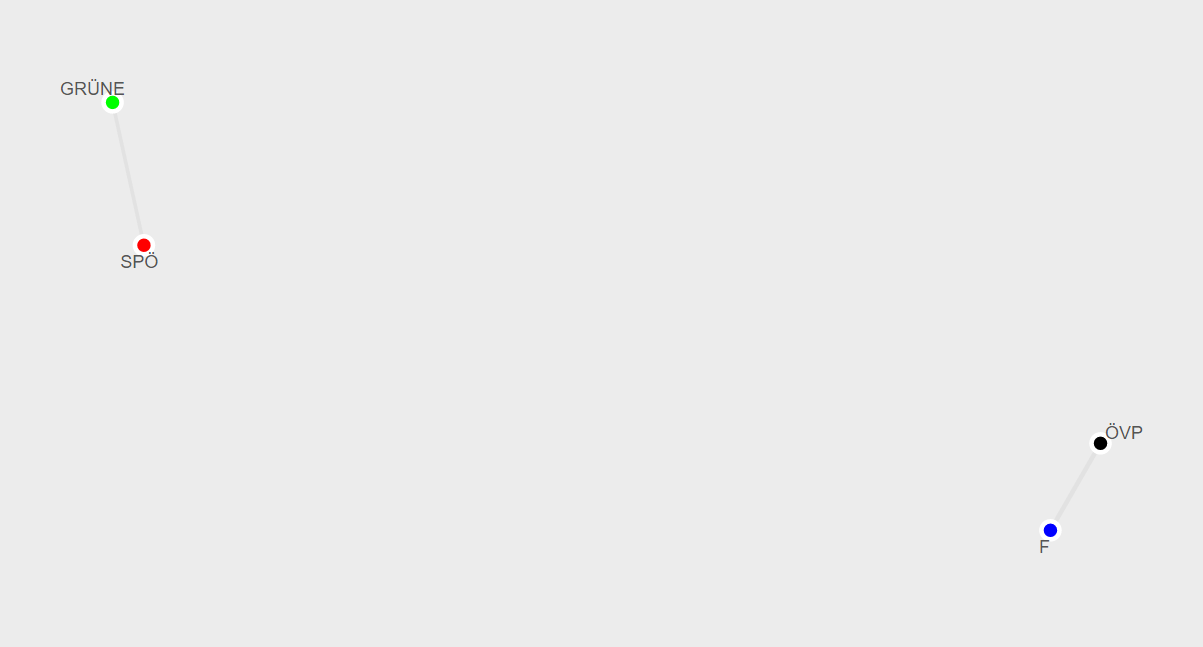
\includegraphics[width=0.49\textwidth]{imgs/graphs/club-graphs/clubs_21} & 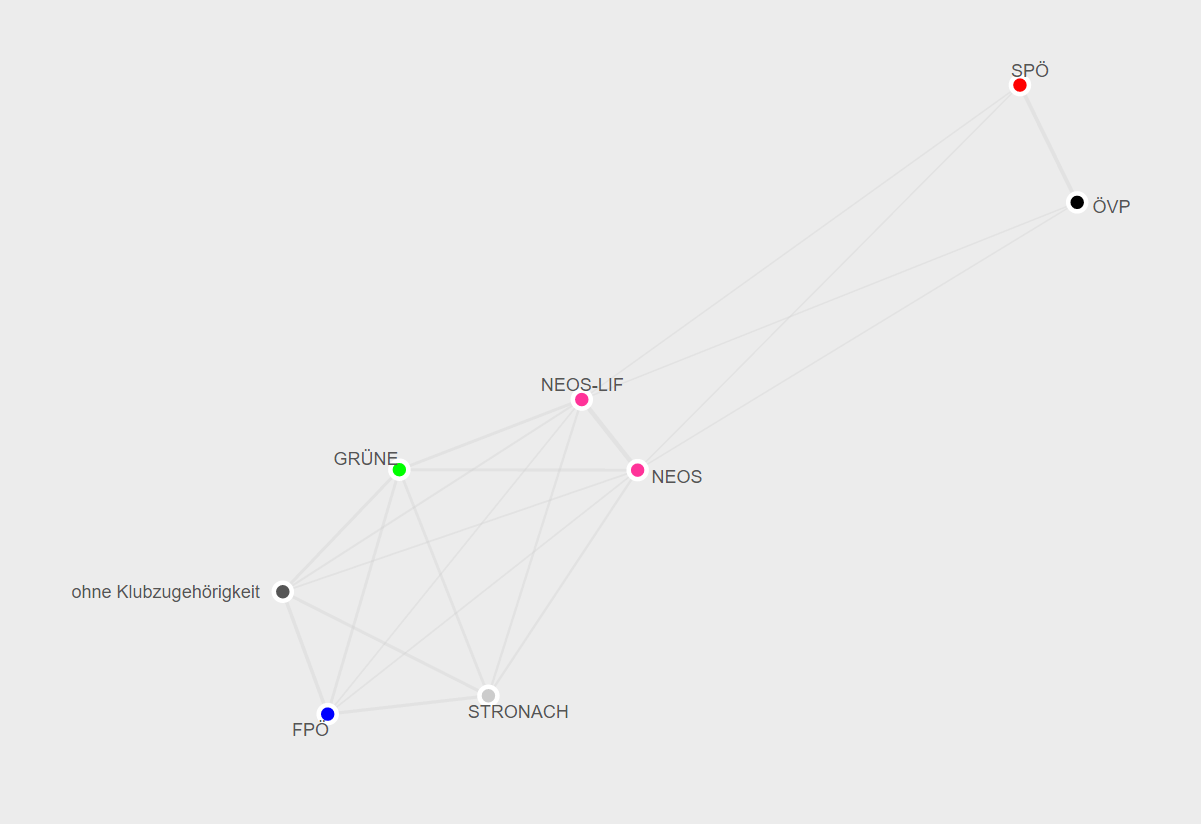
\includegraphics[width=0.49\textwidth]{imgs/graphs/club-graphs/clubs_25}
\end{tabular}
	\caption{Club ............}
	\label{fig:club_graphs1}
\end{figure}


\section{Relations of Politicians}
Graph + Explanations

\section{Government - Opposition Relation}
\label{sec:gov_opp_relation}

\begin{table}[h]

\centering
\bgroup
\def\arraystretch{1.2}
\begin{tabular}{| p{2cm} | p{5cm} | l |}
\hline
  Legislative Period & Governing Parties & Opposition  \\
\hline
\hline
  20. Period & SPÖ, ÖVP & FPÖ, Grüne, Liberale \\
\hline
  21. Period & ÖVP, FPÖ & SPÖ, Grüne \\
\hline
  22. Period & ÖVP, FPÖ, BZÖ (The BZÖ was in government from $17^{th}$ of April, 2005) & SPÖ, Grüne \\
\hline
  23. Period & SPÖ, ÖVP & FPÖ, Grüne, BZÖ \\
\hline
  24. Period & SPÖ, ÖVP & FPÖ, Grüne, Stronach, BZÖ \\
\hline
  25. Period & SPÖ, ÖVP & FPÖ, Grüne, NEOS, Stronach \\
\hline

\end{tabular}
\egroup
\caption{Government and Opposition in the Legislative Periods 20 to 25}
\label{table:gov_opp_parties}
\end{table}



\begin{table}[h]

\centering
\bgroup
\def\arraystretch{1.2}
\begin{tabular}{| p{2cm} | p{3cm} | p{3cm} | p{3cm} |}
\hline
  Legislative Period & Government-Opposition Relation & Inner Government Relation & Inner Opposition Relation \\
\hline
\hline
  20. Period & -0.85 & +1.00 & +0.86 \\
\hline
  21. Period & -0.695 & +0.985 & +0.908 \\
\hline
  22. Period & -0.567 & +1.00 & +0.938 \\
\hline
  23. Period & -0.382 & +0.994 & +0.765\\
\hline
  24. Period & -0.52 & +1.00 & +0.768\\
\hline
  25. Period & -0.374 & +1.00 & +0.676\\
\hline

\end{tabular}
\egroup
\caption{Government-Opposition Relation, Inner Government- and Inner Opposition Relation for the Legislative Periods 20 to 25}
\label{table:gov_opp_relation}
\end{table}